\documentclass[a3paper, twoside, openany]{book}
\usepackage[utf8]{inputenc}
\usepackage[T1]{fontenc}
\usepackage[italian]{babel}
\usepackage[normalem]{ulem}
\usepackage{textcomp}
\usepackage{array}
\usepackage{amsmath}
\usepackage{amsfonts}
\usepackage{asymptote}
\usepackage{dirtytalk}
\usepackage{gensymb}
%\usepackage{csquotes}
\usepackage{graphicx}
\usepackage{amsthm}
%\usepackage{systeme}
\usepackage[dvipsnames]{xcolor}
\graphicspath{{assets/}}
\newenvironment{riq}
    {\begin{center}
    \begin{tabular}{|p{0.9\textwidth}|}
    \hline\vspace{0.5pt}}
    { \vspace{5pt}
    \\\hline
    \end{tabular}
    \end{center}
    }
\theoremstyle{definition}
\newtheorem{definition}{Definizione}

\title{Studio dei circuiti RC}
\author{Giacomo Fortunato}

\begin{document}
\maketitle
\section{Presentazione}
Mi chiamo \textbf{Giacomo Fortunato} e frequento (ancora per poco) la quinta classe, sezione F, al Liceo Scientifico Statale \say{G. Battaglini}. Questo è il mio elaborato di \textbf{Matematica e Fisica} preparato per la simulazione del colloquio d'esame (a.s. 2019/2020, anche noto come anno del COVID). \\ In questa breve relazione percorreremo le strade matematiche di integrali e limiti per studiare il funzionamento dei circuiti RC (a corrente continua), in particolare il comportamento del \textbf{condensatore}. \\ Spero che l'elaborato possa essere di Vostro gradimento, buona lettura.
\section{Strumenti utilizzati}
Questo documento è stato creato utilizzando un linguaggio di markup per la preparazione di testi chiamato \LaTeX\footnote{https://www.latex-project.org}: questo linguaggio è utilizzato continuamente nella produzione di documenti, tesi, relazioni e pubblicazioni di ogni genere, particolarmente di carattere scientifico. Personalmente, scrivo e compilo (trasformare da file codice a file finale) \LaTeX con Atom\footnote{https://atom.io}, l'IDE sviluppato da GitHub\footnote{https://github.com}. (Più tecnicamente, utilizzo \textbf{TeX Live 2019} o \textbf{TeX Live 2020}\footnote{https://tug.org/texlive} e, su Atom, utilizzo il pacchetto \textbf{atom-latex} di @thomasjo\footnote{https://github.com/thomasjo/atom-latex}, e il pacchetto \mbox{\textbf{latex-language2e}} di @Aerijo\footnote{https://github.com/Aerijo/language-latex2e}.) \\ Ho appreso di \LaTeX dai miei compagni più grandi delle Olimpiadi di Matematica, e sono fiero di aver imparato così tanto successivamente da solo. \\ Per i diagrammi, ho utilizzato diagrams.net\footnote{https://www.diagrams.net}, un programma javascipt e web-based per la realizzazione di diagrammi. Il software è open-source\footnote{https://github.com/jgraph/drawio} rilasciato sotto Licenza Apache 2.0\footnote{https://github.com/jgraph/drawio/blob/master/LICENSE}.
\chapter{Dimostrazione iniziale}
\section{Introduzione e premesse}
\begin{figure}[htp]
    \centering
    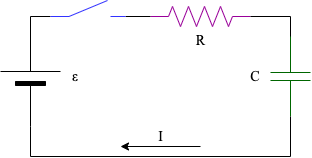
\includegraphics[width=10cm]{Circuito RC-Aperto}
    \caption{Circuito RC aperto}
    \label{fig:RC-aperto}
\end{figure}
Putroppo le condizioni attuali ci impediscono di esplorare troppo a fondo le radici di questo circuito. Tuttavia sarebbe altrettanto sbagliato studiare un circuito RC (figura \ref{fig:RC-aperto}) senza definire poche e semplici definizioni basilari sui circuiti.
\theoremstyle{definition}
\begin{definition}{\textbf{Circuito a corrente continua}}
Un percorso chiuso che viene percorso da una carica, e questa ritorna al suo punto di partenza, è un circuito elettrico a corrente diretta. Sono denominati anche circuiti DC (dall'inglese \emph{Direct Current}).
\end{definition}
\begin{definition}{\textbf{Batteria}}
Una batteria è un dispositivo capace di produrre una differenza di potenziale elettrico ($\Delta V$) ai suoi estremi.
\end{definition}
\begin{definition}{\textbf{Forza elettromotrice indotta, \emph{fem} ($\varepsilon$)}}
La forza elettromotrice indotta è la differenza di potenziale elettrico quando la batteria non genera corrente. Si indica con $\varepsilon$ e si misura in Volt [V].
\end{definition}
\begin{figure}[htp]
    \centering
    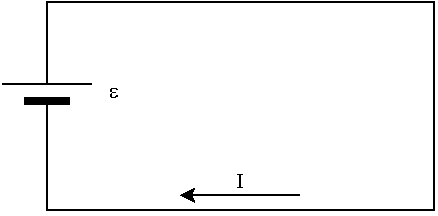
\includegraphics[width=6cm]{Circuito RC-Batteria}
    \caption{Circuito DC con batteria}
    \label{fig:batteria}
\end{figure}
Il filo di un qualunque circuito genera una resistenza al movimento degli elettroni, come se fosse una forma di attrito degli elettroni.
\begin{definition}{\textbf{Resistenza di un filo e prima legge di Ohm}}
La costante di proporzionalità diretta tra la differenza di potenziale $V$ l'intensità di corrente $I$ è la resistenza del filo $R$. Enunciamo quindi la prima legge di Ohm:$$V=IR$$ La resistenza di un filo si misura in Omh ($\Omega$). Nel modello fisico, se il filo è una linea dritta, la resistenza in quella parte di filo è nulla; per indicare la resistenza in un filo si usa il simoblo in viola nella figura \ref{fig:resistenza}.
\end{definition}
\begin{figure}[htp]
    \centering
    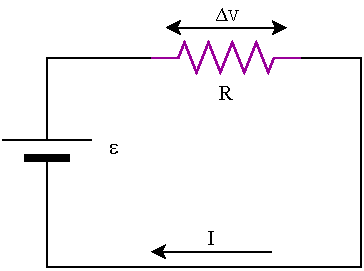
\includegraphics[width=6cm]{Circuito RC-Resistenza}
    \caption{Circuito DC con batteria e resistenza}
    \label{fig:resistenza}
\end{figure}
\begin{definition}{\textbf{Capacità di un condensatore}}
Un condensatore è un dispositivo dotato di due facce piane chiamate armature capaci di accumulare carica elettrica: su una faccia accumula una carica positiva $+q$, sull'altra una carica negativa $-q$ (in verde nelle figure \ref{fig:condensatore}, \ref{fig:condensatore-z} e \ref{fig:condensatore-3d}). \\ La carica di un condensatore $Q$ è direttamente proporzionale alla differenza di potenziale $V$, e questo rapporto è la caratteristica del condensatore, la sua capacità. $$C=\frac{Q}{V}$$ La capacità di un condensatore si misura in Farad (F) (che sarebbe Coulomb su Volt).
\end{definition}
\begin{figure}[htp]
    \centering
    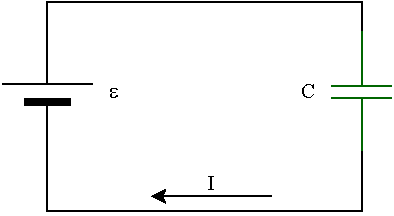
\includegraphics[width=6cm]{Circuito RC-Condensatore}
    \caption{Circuito DC con batteria e condensatore}
    \label{fig:condensatore}
\end{figure}
\begin{figure}[htp]
    \centering
    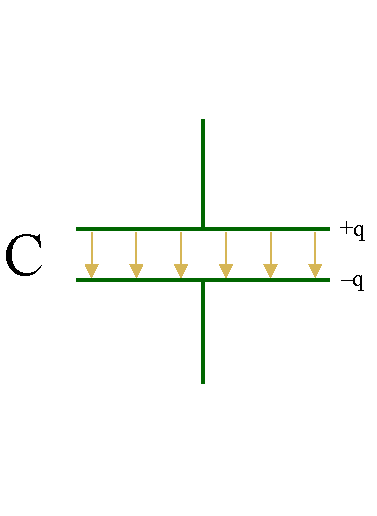
\includegraphics[width=6cm]{Circuito RC-Condensatore-zoom}
    \caption{Ingrandimento del condensatore}
    \label{fig:condensatore-z}
\end{figure}
\begin{figure}[htp]
    \centering
    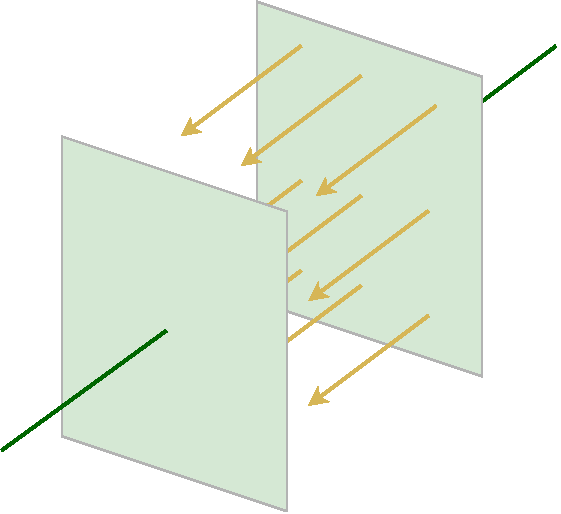
\includegraphics[width=6cm]{Circuito RC-Condensatore-3D}
    \caption{Modello tridimensionale di un condensatore}
    \label{fig:condensatore-3d}
\end{figure}
\begin{definition}{\textbf{Legge dei nodi di Kirchhoff}}
Presupposto che un nodo è un punto del circuito in cui si incontrano 3 o più fili, la somma algebrica di tutte le correnti che convergono in un nodo di un circuito deve essere uguale a 0. Se la corrente esce dal nodo l'intesità sarà di segno negativo, se la corrente entra nel nodo l'intenistà sarà di segno positivo. $$\text{In nodo:}\sum{I_n}=0$$ Nella figura \ref{fig:nodo}, $|I_1+I_2|=|I_3|$, ma in particolare: $$I_1+I_2=-I_3\longrightarrow I_1+I_2+I_3=0$$
\end{definition}
\begin{figure}[htp]
    \centering
    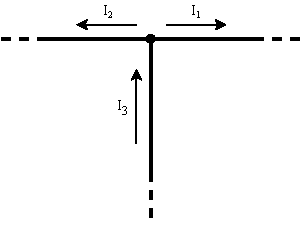
\includegraphics[width=6cm]{Circuito RC-Nodo}
    \caption{Esempio di nodo con intensità di corrente segnate}
    \label{fig:nodo}
\end{figure}
\begin{definition}{\textbf{Legge delle maglie di Kirchhoff}}
Presupposto che una maglia è un qualsiasi segmento di circuito chiuso (compreso tra 2 nodi), la somma algebrica di tutte le differenze di potenziale lungo una maglia di un circuito è uguale a 0. Poiché in ogni circuito dove scorre corrente, è necessariamente presente una batteria, formalizziamo: $$\varepsilon+\sum{\Delta V}=0\longleftrightarrow \varepsilon=-\sum{\Delta V}$$
\end{definition}
\begin{figure}[htp]
    \centering
    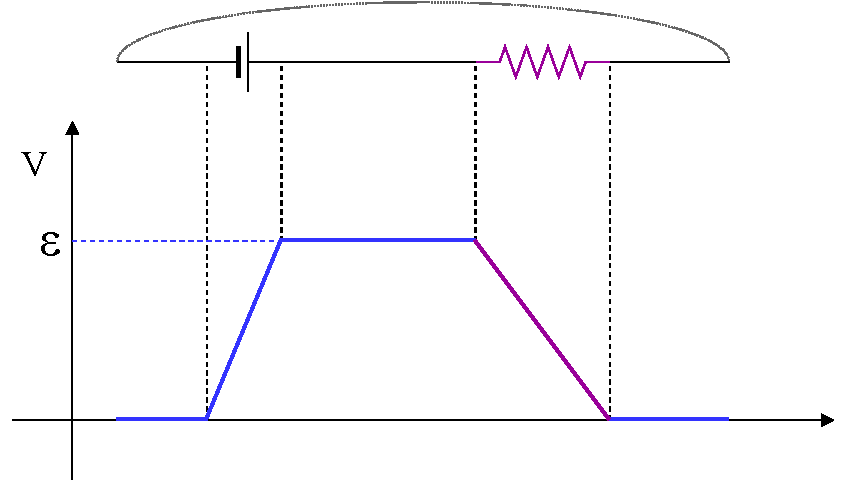
\includegraphics[width=10cm]{Circuito RC-Maglia}
    \caption{Grafico dell'andamento del potenziale in un circuito DC}
    \label{fig:maglia}
\end{figure} \clearpage
\section{Circuiti RC}
\begin{figure}[htp]
    \centering
    \includegraphics[width=10cm]{Circuito RC-chiuso}
    \caption{Circuito RC chiuso}
    \label{fig:RC-chiuso}
\end{figure}

Nella figura \ref{fig:RC-aperto}, ho mostrato subito un circuito RC aperto, cioé un cicuito dove sono inseriti una batteria, una resistenza e un condensatore in serie. \\ Se in un circuito con solo batteria e condensatore, viene chiuso un interrutore (in blu nella figura \ref{fig:RC-aperto}), le armature dei condensatori si caricano quasi istantaneamente. In un circuito RC invece la resistenza limita la velocità di propagazione delle cariche e può passare un certo tempo prima che i condensatori comincino davvero a caricarsi. Questo fenomeno è il concetto chiave di questo elaborato.
\subsection{Carica del condensatore nel circuito RC}
Prima dell'istante $t=0$, il circuito è aperto, esattamente come in figura \ref{fig:RC-aperto}. Esattamente nell'istante $t=0$, il circuito viene chiuso (figura \ref{fig:RC-chiuso}), e viene permesso alla corrente di attraversare il circuito: è da questo istante che inizia l'esperienza. \\ Consideriamo $V(t)$ la differenza di potenziale $V$ del condensatore in funzione del tempo $t$, e consideriamo $Q(t)$ la carica $Q$ del condensatore in funzione del tempo $t$. Per cui: $$t=0\longrightarrow V(t)=0 \wedge Q(t)=0$$ Procediamo \emph{step by step}:
\begin{enumerate}
\item Per la definizione di intensità di corrente elettrica $I$, questa stessa sarà: \begin{equation}\textcolor{blue}{I}=\lim_{t\mapsto 0}\frac{\Delta Q(t)}{\Delta t}=\textcolor{blue}{\frac{dQ}{dt}}\end{equation}
\item Studiamo la capacità $C$ del nostro condensatore: \begin{equation}C=\frac{Q(t)}{V(t)}\longleftrightarrow \textcolor{Green}{V(t)=\frac{Q(t)}{C}}\end{equation}
\item Ora \emph{incolliamo questi elementi in un collage} grazie alla \textbf{legge di Ohm} e la \textbf{legge delle maglie di Kirchhoff}: \begin{equation}\varepsilon-V(t)=V,V=IR,\varepsilon-\textcolor{Green}{V(t)}=\textcolor{blue}{I}R***\end{equation} \begin{equation}\varepsilon-\textcolor{Green}{\frac{Q(t)}{C}}=R\textcolor{blue}{\frac{dQ}{dt}}\end{equation}
\item Riarrangiamo l'equazione: \begin{equation}dt=\frac{RC\,dQ}{\varepsilon C-Q}\end{equation}
\item In questo momento è neccesario risolvere l'eqauzione differenziale che abbiamo ottenuto. È neccesaria una mossa molto scaltra, una sostituzione di variabile efficace, che influenzi positivamente non solo la variabile stessa ma anche il differenziale di questa: \begin{equation}x=\varepsilon C-Q\;\;\;\;\;dQ=-dx\end{equation} Questa sostituzione è fondamentale per non modificare l'equazione in alcun modo, mascherandola però in un'equazione differenziale che sappiamo risolvere.***
\item Sostituiamo e integriamo entrambi i membri dell'equazione: \begin{equation}dt=\frac{RC}{x}dx\longrightarrow \int_0^tdt=-RC\int_0^t\frac{dx}{x}\longrightarrow t=-RC\ln{\left(\frac{x(t)}{x(0)}\right)}\end{equation}
\item Risolviamo rispetto a $x(t)$: \begin{equation}x(t)=-x(0)e^{-\frac{t}{RC}}\end{equation}
\item Applichiamo la sostituzione (1.6) inversa e ordiniamo l'equazione finale: \begin{equation}\begin{split}\varepsilon C-Q(t)=\varepsilon Ce^{-\frac{t}{RC}} \\ Q(t)=\varepsilon C \left(1-e^{-\frac{t}{RT}}\right)\end{split}\end{equation}
\end{enumerate} Siamo arrivati a una conclusione molto interessante: per facilitare la comprensione, colorerò tutti gli elementi caratterizzanti che dipendono dal circuito e lascerò in nero solo gli elementi fissi e la variabile $t$, che è la variabile della funzione che stiamo studiando: $$\textcolor{blue}{Q}(t)=\textcolor{orange}{\varepsilon}\textcolor{Green}{C}\left(1-e^{-\frac{t}{\textcolor{Purple}{R}\textcolor{Green}{C}}}\right)$$
\subsection{Studio della carica del condensatore}
Per confermare questo risultato, effettuiamo una prova: se $t=0,\longrightarrow Q(t)=0$ come scritto nella premessa della dimostrazione. Proviamo sfruttando il limite della funzione. Il limite per $t$ che tende a 0 è semplice, poiché siamo in grado di garantire che la funzione sia continua nel suo dominio, cioé $[0;+\infty)$, e grazie alle proprietà della continuità***, possiamo calcolare il limite: \begin{multline*}\lim_{t\mapsto 0}Q(0)=\varepsilon C \left(1-e^{-\frac{0}{RC}}\right)\longrightarrow \lim_{t\mapsto 0}Q(0)=\varepsilon C \left(1-e^{-0}\right)\longrightarrow \\\longrightarrow \lim_{t\mapsto 0}Q(0)=\varepsilon C (1-1)\longrightarrow \lim_{t\mapsto 0}Q(0)=\varepsilon C 0=0\end{multline*} Ottimo! Abbiamo vinto! \\ Avendo iniziato a studiare, calcoliamo ora il limite con $t$ che tende verso più infinito: \begin{multline*}\lim_{t\mapsto +\infty}Q(t)=\varepsilon C \left(1-e^{-\frac{\infty}{RC}}\right)\longrightarrow \lim_{t\mapsto +\infty}Q(t)=\varepsilon C \left(1-e^{-\infty}\right)\longrightarrow \\\longrightarrow \lim_{t\mapsto +\infty}Q(t)=\varepsilon C (1-0)\longrightarrow\lim_{t\mapsto +\infty} Q(t)=\varepsilon C\end{multline*} Cosa vuol dire? Vuol dire che, se lasciamo il circuito chiuso per un lungo periodo di tempo, la carica del condensatore si avvicinerà sempre di più al valore di $\varepsilon C$, tuttavia non potrà mai essere esattamente quel valore o superarlo. Possiamo concludere questo limite dicendo che la \textbf{carica massima di un condensatore} in un circuito RC è $\varepsilon C$. La forma bizzara dell'equazione ci suggerisce un ultimo esperimento: il valore della carica se $t=RC$: il prodotto $RC$ è a tutti gli effetti una misura di tempo, come dimostrato dall'analisi dimensionale:
$$[R][C]=\frac{[V][t]}{[Q]}\cdot\frac{[Q]}{[V]}=\frac{[\xout{V}][t]}{[\xout{Q}]} \cdot \frac{[\xout{Q}]}{[\xout{V}]}=[t]$$ Questo elemento si chiama \textbf{costante di tempo} (o tempo caratteristico) del circuito RC e si indica con $\tau$. Se $t=\tau$, come si comporta la carica del condensatore? $Q(\tau)=0,632\,\varepsilon C$, o, per essere ancora più precisi, $Q(t)=\left(1-e^{-1}\right) \varepsilon C$. Grazie alla potenza dei calcolatori e dei programmi di \emph{plotting}, siamo capaci di visualizzare con facilità estrema i grafici di tutte le funzioni: ecco come nel grafico della figura \ref{fig:carica} possiamo confermare il dato matematico del limite, con un asintoto orizzontale $y=\varepsilon C$.
\begin{figure}[htp]
    \centering
    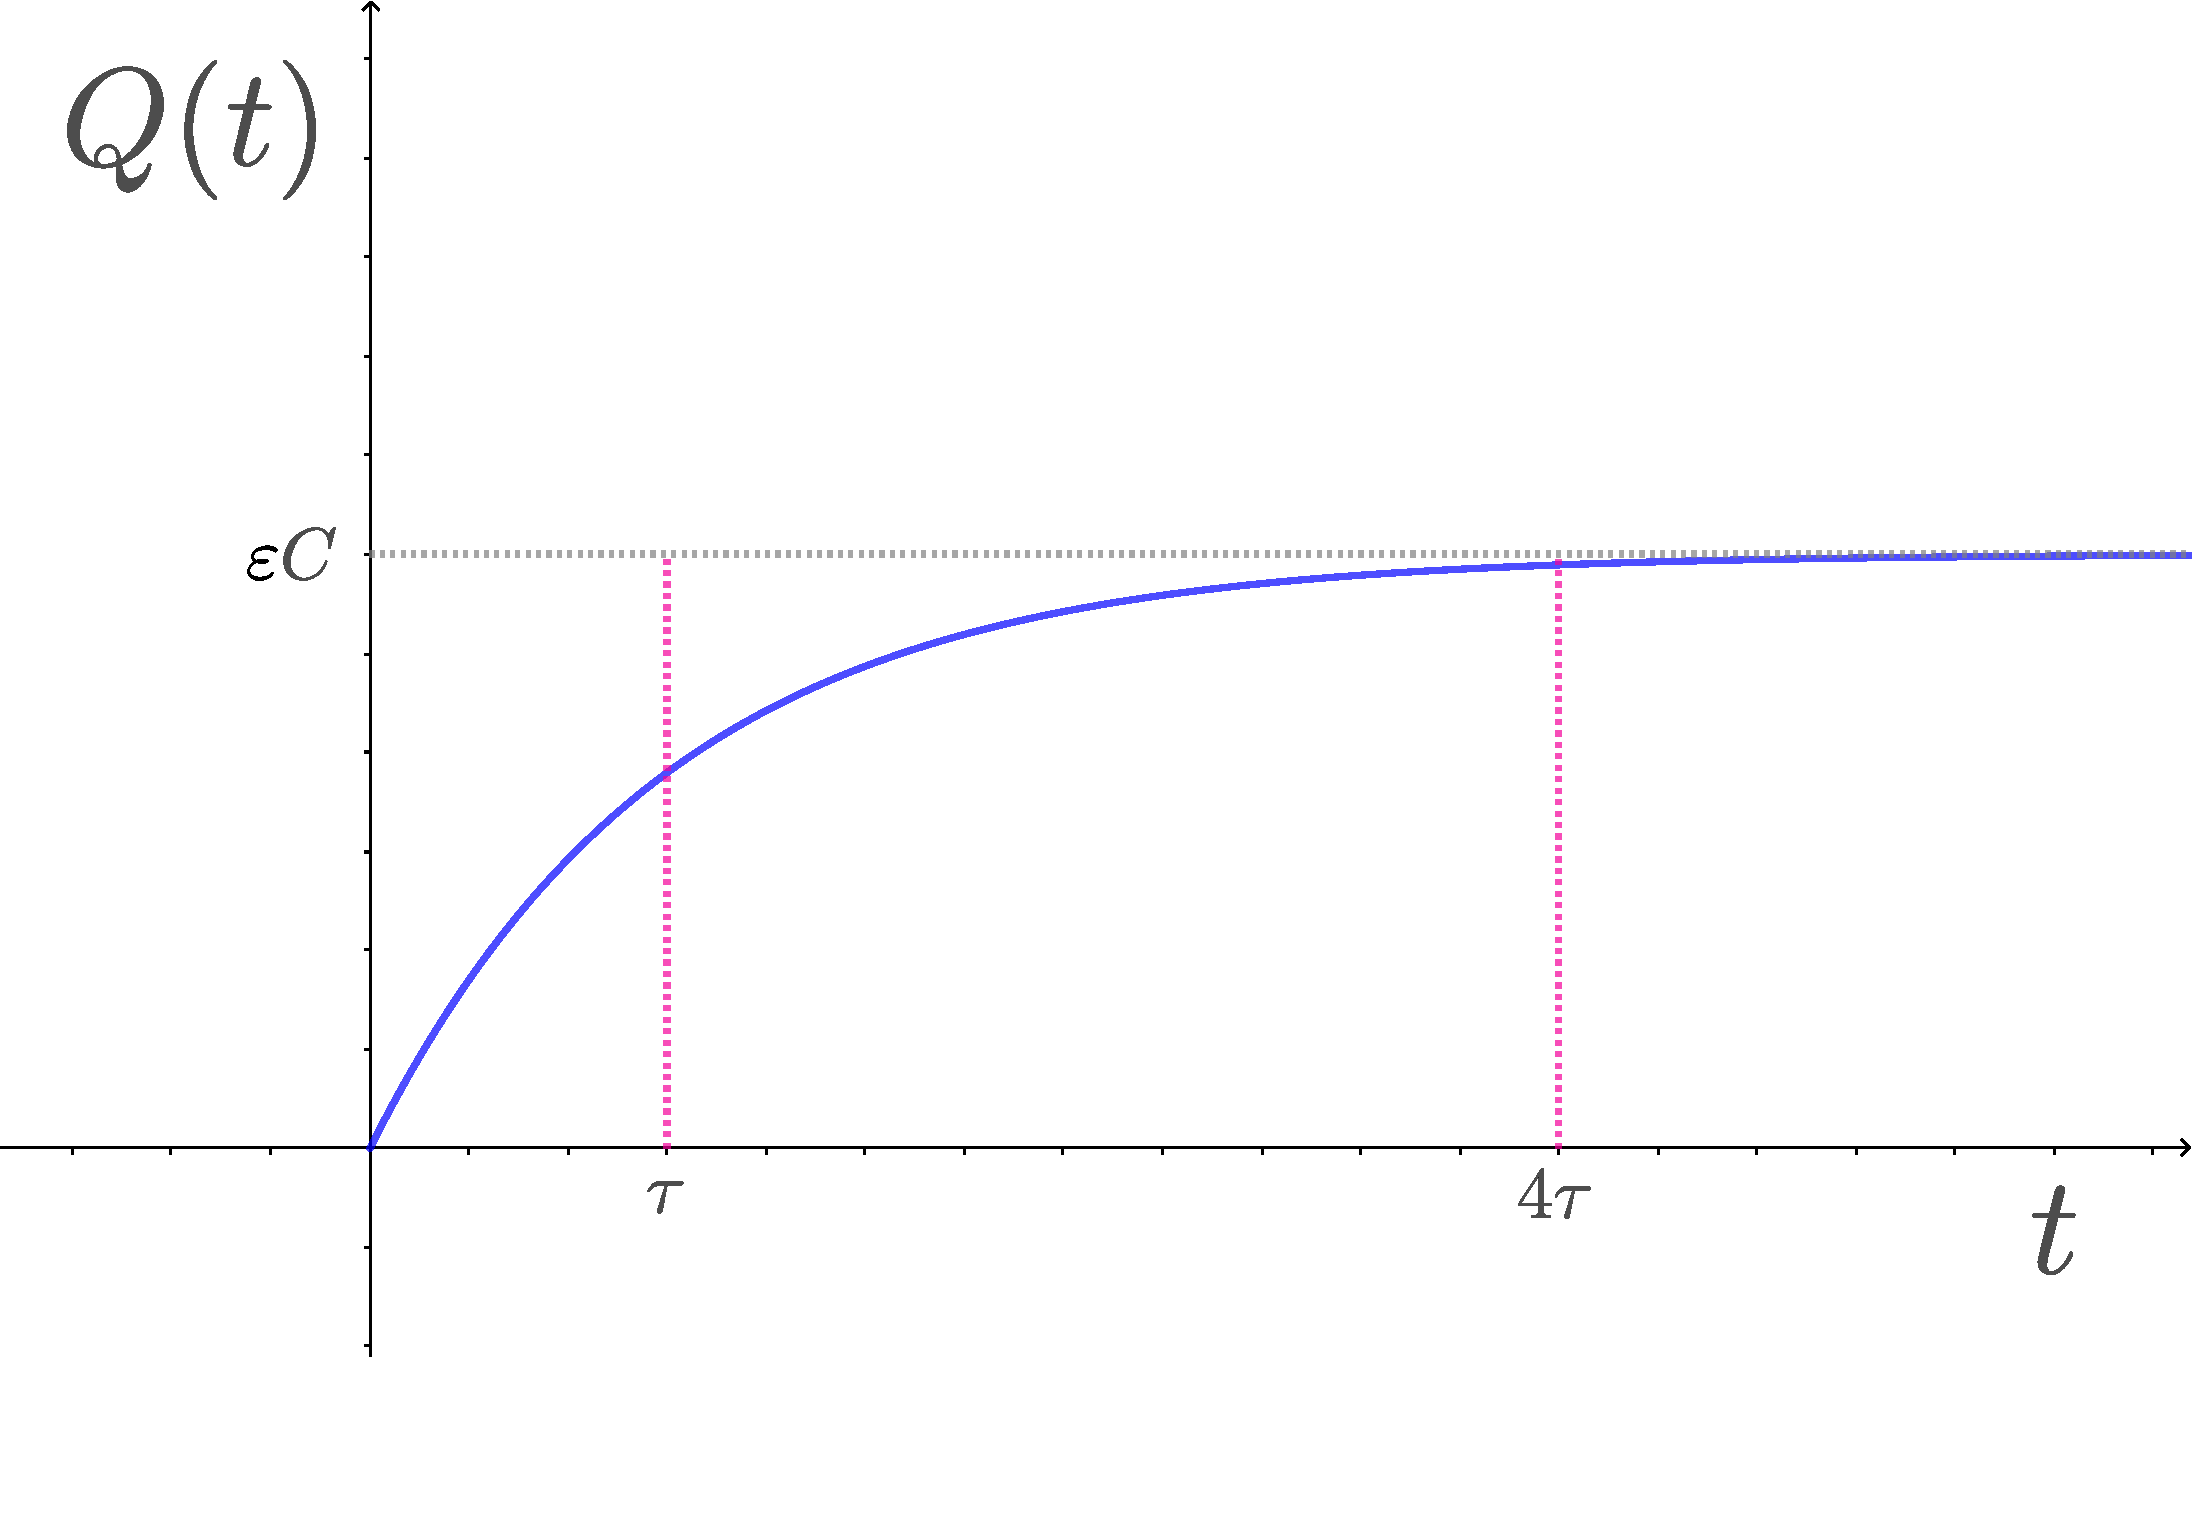
\includegraphics[width=10cm]{Carica}
    \caption{Grafico della carica di un condensatore}
    \label{fig:carica}
\end{figure}









\end{document}
